This chapter provides a brief overview of suspension system history and development, followed by reviewing the most recent studies concerned with modern control techniques in Active suspension system.

\section{Suspension system history}
Suspension is the term given to the system that connects a vehicle body to its wheels and allows relative motion between them. This Relative motion between the wheel and the body is necessary to isolate the vehicle's body from the road irregularities that are fed into the tire at the road/wheel interface. In general, some kind of linkage system that combines damping and stiffness controls this motion. We refer to this process as a suspension. This Damping and stiffness are fed to the system through the dampers, springs (shock absorbers) and the linkages that transmit motion or forces between various parts of the suspension system. \cite{alashtari2023fuzzy}, \cite{barton2018automotive}

In the 15$^{\text{th}}$ century, people understood that suspensions were crucial for making passengers feel comfortable.
Back then, coaches had bodies that hung from a set of leaf springs attached to a strong chassis. This chassis held the wheel hubs. The loose ends of the springs were linked to the coach's body using leader belts. Figure \ref{fig:coach} shows a coach\cite{oliver1981} from around 1650 with this kind of suspension setup, providing a fascinating example. \cite{genta2014motorcar} \cite{anfia2010}

\begin{figure}[H]
	\centering
	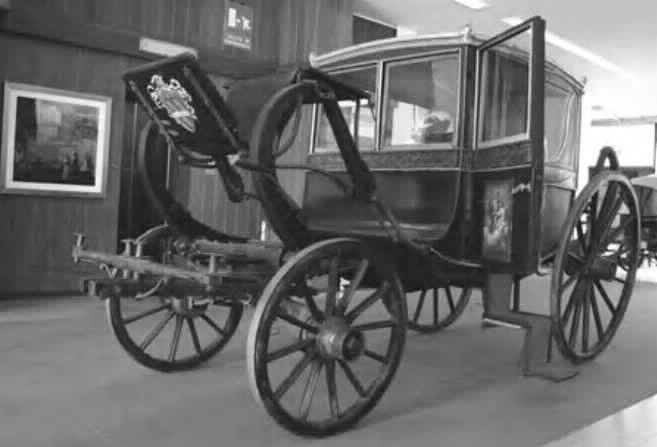
\includegraphics[width=0.4\textwidth]{2.1.png}
	\caption{This coach, built around 1650, shows a suspension made by four leaf springs and leader belts (National Automobile Museum of Torino). \cite{genta2014motorcar}
	}
	\label{fig:coach}
\end{figure}


\subsection{Suspension system evolution}
\begin{enumerate}
	\item \textbf{Passive Suspension Systems (Before 1980s):}
	\begin{itemize}
		\item Early automotive suspension systems were mostly passive, relying on mechanical components such as springs and dampers to absorb shocks and vibrations.
		\item These systems were simple and cost-effective but offered limited adaptability to varying road conditions.
	\end{itemize}
	\item \textbf{Active Suspension Systems (1980s - 1990s):}
	\begin{itemize}
		
		\item The concept of active suspension, which actively adjusts the suspension settings in response to changing road conditions, gained popularity in the 1980s.
		\item One of the pioneering examples was the development of the Lotus Active Suspension in Formula 1 in the late 1980s.
		\item Some high-end road cars began to incorporate active suspension systems in the late 1980s and early 1990s, including models from manufacturers like Citroën and Cadillac.
		\item Active suspension systems used sensors to monitor various factors, and electronic control systems adjusted the suspension settings in real-time to optimize ride comfort and handling.
	\end{itemize}
	
	\item \textbf{Semi-Active Suspension Systems (1990s - Present):}
	\begin{itemize}
		
		\item Semi-active suspension systems represent a middle ground between passive and active systems.
		\item In a semi-active system, the suspension settings are adjusted in real-time, but they typically do not provide as much active control as fully active systems.
		\item Popular semi-active systems include electronically controlled shock absorbers (e.g., Delphi's MagneRide) that can adjust damping rates based on driving conditions.
		\item These systems offer improved ride quality and handling without the complexity and cost associated with fully active systems.
	\end{itemize}
	
	\item \textbf{Recent Developments (2000s - Present):}
	\begin{itemize}
		
		\item Advancements in sensor technology, computing power, and materials have allowed for more sophisticated suspension systems.
		\item Active and semi-active suspension systems continue to evolve, with a focus on enhancing performance, safety, and comfort.
		\item Some modern high-performance and luxury vehicles feature advanced adaptive suspension systems that can adjust multiple parameters, including ride height, stiffness, and damping rates.
	\end{itemize}
\end{enumerate}
The semi-, figure \ref{fig:semi and active} (a), and fully-, figure \ref{fig:semi and active} (b), active suspension system are introduced. \cite{alashtari2023fuzzy}

\begin{figure}[H]
	\centering
	\begin{subfigure}{.35\textwidth}
		\centering
		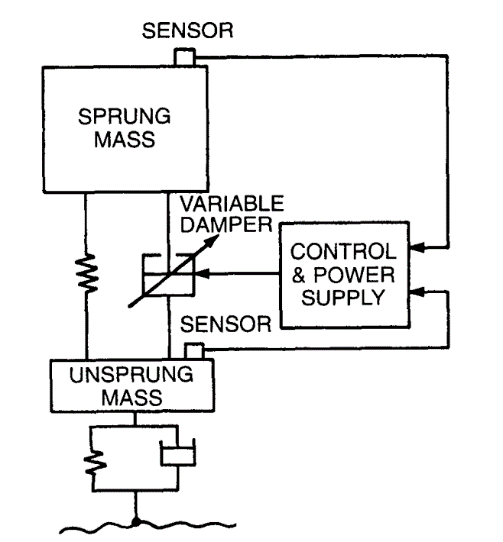
\includegraphics[width=\textwidth]{semi.png}
		\subcaption*{(a)}
	\end{subfigure}%
	\begin{subfigure}{.35\textwidth}
		\centering
		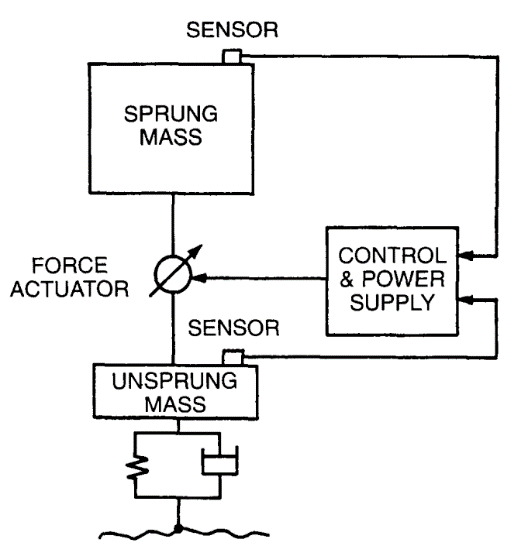
\includegraphics[width=\textwidth]{active.png}
		\subcaption*{(b)}
	\end{subfigure}
	\caption{Schematics of (a) Semi-active and (b) Fully-active suspension systems \cite{wong2001theory}}
	\label{fig:semi and active}
\end{figure}

Active suspension system is even beneficial for the HVG (Heavy Goods Vehicle) in case of the vehicle negotiating a turn.

\begin{figure}[H]
	\centering
	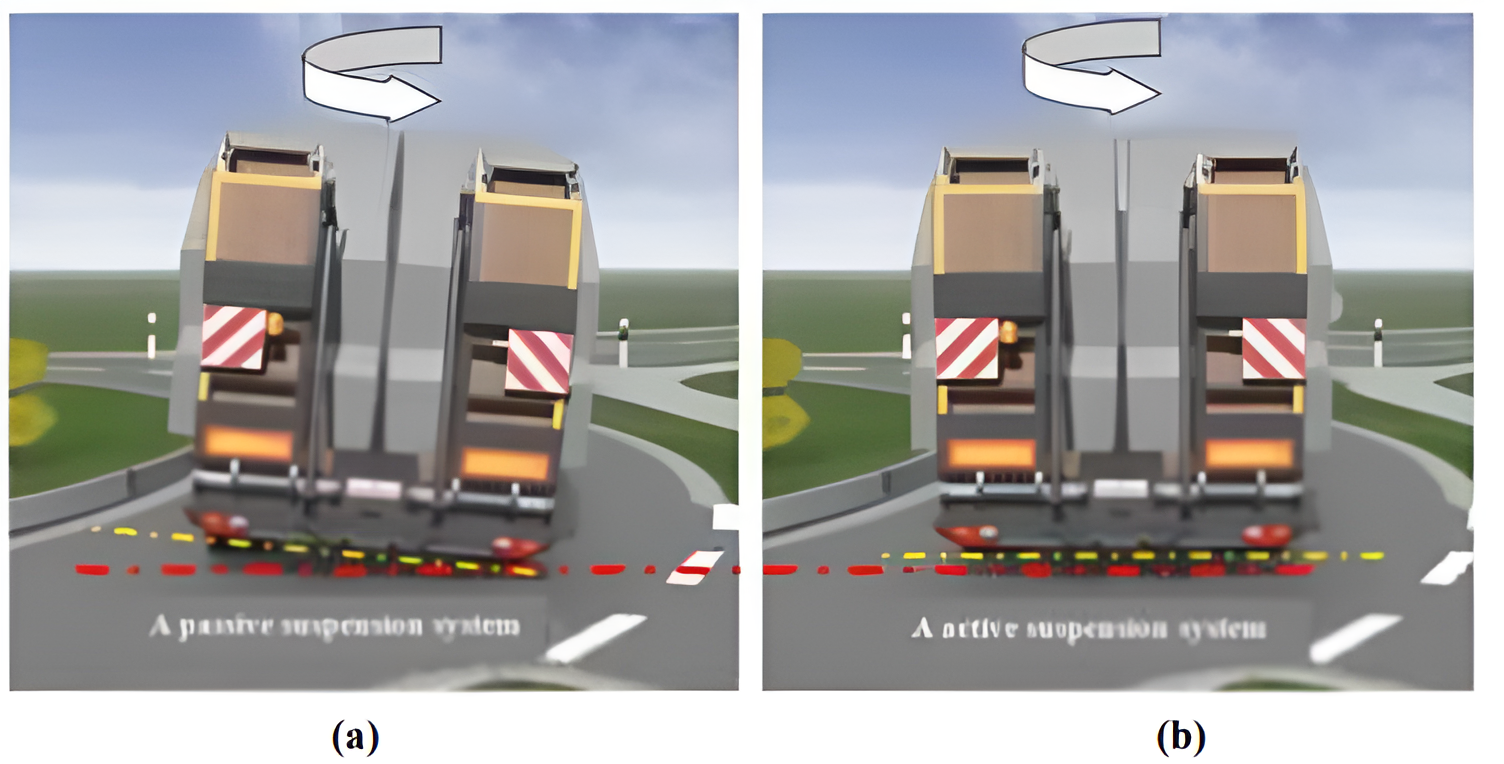
\includegraphics[width=.4\linewidth]{rolldef.png}
	\caption{Difference between the behavior of the truck body in a curve: with passive suspension (a) and with active suspension (b). \cite{hamza2022intelligent}}
	\label{fig:rolldef}
\end{figure}

\section{Recent Research}
\subsection{PID controller}
Many studies have explored various control strategies for active suspension systems over the last few decades. One of the commonly used approaches is the PID (Proportional-Integral-Derivative) algorithm, which was employed by \cite{duong2022modeling} to control the dynamics of active suspension systems. The PID controller operates in three distinct stages, each corresponding to one of the three tuning coefficients: $K_p$ (proportional), $K_D$ (derivative), and $K_i$ (integral). These coefficients can either be self-tuned through adaptive techniques or selected using standard methods like Ziegler-Nichols’s method, which is a heuristic approach to tuning PID controllers based on system response characteristics \cite{huba2021making}. This method helps achieve a balance between the system's stability and response speed.

However, the effectiveness of PID controllers often suffers from limitations in complex or nonlinear systems, where manual tuning or standard methods may not yield optimal results. To address these challenges, alternative approaches have been explored. For instance, \cite{chen2018modelling} applied the Fuzzy logic algorithm to tune the PID controller’s variables dynamically based on real-time excitation signals from the road. Fuzzy logic controllers can handle imprecision and uncertainty, offering a more adaptable solution in environments with unpredictable disturbances. Another advanced approach involves using Genetic Algorithms (GA) to optimize the PID controller’s parameters. The GA, based on principles of natural selection and genetics, can search for optimal parameter values by evaluating fitness over successive generations. This technique was demonstrated by \cite{metered2018optimized}, who applied it to fine-tune the PID controller. The GA solution allows for more flexibility in choosing optimal values for $K_p$, $K_D$, and $K_i$, adjusting to varying system conditions. The size of the population and the number of generations required for convergence are typically determined by the designer’s experience and the complexity of the system.

In contrast to the GA, the Particle Swarm Optimization (PSO) method offers another optimization technique inspired by the social behaviors of animals. PSO mimics the flocking behavior of birds or the schooling behavior of fish, where individual particles (agents) adjust their positions based on their own experience and the collective experience of their neighbors. This swarm-based approach was used by \cite{al2015quarter} to optimize the PID controller’s coefficients. The PSO algorithm is particularly useful for problems with a large number of variables and complex search spaces, as it can efficiently explore the solution space without requiring detailed knowledge of the system’s underlying dynamics.

Moreover, numerous other intelligent algorithms, such as Ant Colony Optimization (ACO) and Bee Colony Optimization (BCO), have also been explored for the optimal search of controller parameters. These bio-inspired algorithms exhibit strong performance in dynamic optimization problems, as they can adjust to system changes over time \cite{dahunsi2020proportional+}. These algorithms, like PSO and GA, offer robust alternatives to traditional optimization techniques by incorporating flexibility and adaptability.

However, when dealing with complex systems involving multiple controlled objects, a single PID controller might not be sufficient to handle all the required parameters simultaneously. In such cases, one solution is to use multiple PID controllers, each responsible for controlling different aspects or subsystems of the overall system. \cite{nguyen2021improving} explored this approach, where multiple PID controllers were used in parallel to handle the multiple degrees of freedom in an active suspension system. This method can improve performance by distributing the control efforts across different subsystems, thus ensuring better overall system behavior.

\subsection{LQR controller}
The Linear-Quadratic Regulator (LQR) controller is increasingly used to replace conventional Proportional-Integral-Derivative (PID) controllers, particularly in Multi-Input Multi-Output (MIMO) systems where multiple variables need to be controlled simultaneously \cite{wu2021multi}. The key advantage of the LQR controller lies in its ability to optimize the system’s performance by minimizing a predefined cost function, thereby improving the stability and efficiency of the system \cite{rodriguez2021active}. The optimization process involves minimizing a cost function that balances both state variables and control inputs, ensuring the system's behavior is optimal. To implement the LQR controller, the system’s mathematical model must be represented in state-space form, where the system dynamics are captured by a set of linear differential equations expressed as a state matrix \cite{nguyen2022application}. This allows for the precise calculation of the control input that minimizes the cost function at any given time.

A significant extension of the LQR controller is the Linear-Quadratic-Gaussian (LQG) controller, which combines the LQR framework with a Gaussian filter. The LQG controller incorporates the ability to estimate system states in the presence of noise and uncertainty, making it more robust in real-world applications. By combining state estimation techniques, such as Kalman filtering, with LQR control, the LQG controller can address uncertainties in system modeling and measurement, providing better control performance in dynamic environments \cite{xia2015linear}.

Recent advancements in Linear Quadratic Regulator (LQR) control have contributed significantly to the evolution of control theory, leading to improvements in both stability and applicability. One of the notable developments is the revisitation of the LQR problem for singular systems. Researchers have focused on extending the traditional LQR techniques to handle singular systems, where the system dynamics are not fully controllable or observable in the standard sense. These singular LQR techniques help broaden the applicability of LQR controllers to more complex and unconventional systems \cite{lqr_singular_systems}.

Furthermore, the role of predictions in enhancing LQR performance has been explored, especially in online control scenarios under stochastic and adversarial disturbances. By incorporating predictive models, LQR controllers can anticipate future system states and adjust the control actions proactively, improving the system's robustness against uncertainties and disturbances \cite{lqr_predictions}. In addition, data-driven approaches have gained traction, with researchers proposing LQR frameworks that rely on recursive learning algorithms and policy gradient methods. These data-driven LQR frameworks not only ensure stability but also allow the system to adapt to changing conditions by learning from past experiences, making them suitable for modern, adaptive control systems \cite{lqr_stability_recursive}.
	
\textbf{The above methods are only used for linear objects. If the object is nonlinear, more complex algorithms need to be used such as SMC MPC and RL.}




\subsection{SMC controller}
The Sliding Mode Control (SMC) algorithm is widely used for controlling complex nonlinear systems due to its robustness and ability to handle uncertainties and disturbances effectively \cite{meetei2021enhanced}. Kazemian et al. applied the SMC algorithm to control hydraulic actuators, which are commonly used in active suspension systems for their ability to provide precise force control. However, to simplify the modeling of the hydraulic actuator and make the control design more tractable, a linearization process is often performed. This process, which helps approximate the nonlinearities of the actuator, was outlined by Nguyen \cite{nguyen2021advance}. By linearizing the system, it becomes easier to apply traditional control techniques, though it still retains the essential dynamics for practical use. Subsequently, a quarter-dynamic model that considers the influence of the actuator on the vehicle's suspension system is introduced. This model typically involves five state variables, which represent the system's key dynamic parameters, such as displacement, velocity, and force \cite{nguyen2022novel}.

According to Zhao et al. \cite{zhao2023sliding}, the sliding surface plays a crucial role in the effectiveness of the SMC algorithm. The sliding surface is a boundary that separates desirable system states from undesirable ones. In the context of active suspension systems, this surface is used to drive the system’s state to a steady condition, ensuring that the vehicle’s suspension behaves in a stable manner. Once the system reaches the sliding surface, it can travel along this surface to achieve equilibrium, effectively nullifying the impact of disturbances and uncertainties.

A common issue with SMC, however, is the phenomenon known as "chattering." Chattering occurs when the control signal oscillates at high frequencies with small amplitudes, which can lead to undesirable vibrations in the system and potentially cause wear and tear on mechanical components. This issue is particularly problematic in applications like active suspension systems, where smooth control is essential for ride comfort. To mitigate chattering, researchers have proposed combining the SMC algorithm with other control strategies, such as Proportional-Integral-Derivative (PID) controllers or Fuzzy Logic controllers. For instance, Hsiao and Wang \cite{hsiao2022evaluation} introduced an innovative algorithm that integrates SMC with Fuzzy Logic, resulting in a Self-tuning Fuzzy Sliding Mode Controller (STFSMC). The fuzzy logic component allows for adaptive tuning of the control parameters, which helps reduce chattering while maintaining the robustness of the SMC algorithm.

Another approach, suggested by Suhail et al. \cite{suhail2022adaptive}, is the use of the Adaptive Sliding Mode Control (ASMC) algorithm. This method adapts the sliding mode controller in real-time, adjusting its parameters based on the system’s changing conditions. By doing so, it enhances the controller's performance and minimizes the chattering phenomenon. The combination of adaptive control and SMC offers an effective solution to the challenges of controlling nonlinear active suspension systems. Studies have shown that using such advanced control methods significantly improves ride comfort by optimizing the suspension's response to road disturbances \cite{wang2018nonlinear}. Furthermore, numerous other advanced control strategies have been applied to active suspension systems, each bringing high levels of efficiency, adaptability, and precision, making them highly suitable for modern automotive applications.
	
\subsection{RL controller}
Recent advancements in the application of reinforcement learning (RL) for active suspension systems have yielded promising results, particularly in enhancing ride comfort and vehicle stability. Reinforcement learning, with its ability to adapt and optimize in real-time, offers a dynamic approach to controlling active suspension systems. For instance, a study on deep reinforcement learning for active suspension control demonstrates its potential to meet the stringent ISO 2631-5 comfort requirements, which assess human exposure to vibration during vehicle operation \cite{deep_rl_suspension}. This study showcases how deep RL algorithms can effectively minimize vibrations and improve comfort by learning to adjust suspension parameters to various road conditions. Another research effort introduced a TD3-based control algorithm, specifically designed to address actuator delays in active suspension systems. The TD3 algorithm, known for its stability and efficiency in continuous action spaces, proves to be particularly useful in reducing the negative impact of actuator delays on system performance, resulting in better responsiveness and smoother ride quality \cite{td3_active_suspension}.

The optimization of full-vehicle active suspension systems using advanced reinforcement learning controllers has also been extensively explored, leading to significant improvements in both ride comfort and vehicle dynamics. Full-vehicle suspension systems are often subjected to a variety of road irregularities, vehicle loads, and driving conditions, making their control more complex. However, RL controllers, which can learn from these real-world variations, have shown considerable success in optimizing suspension behavior. These controllers can continuously adapt to changing conditions, leading to more efficient suspension responses and improved overall ride comfort \cite{ai_rl_full_vehicle}. Similarly, RL-based vibration control for half-car active suspension systems has demonstrated the effectiveness of adaptive dynamic programming (ADP) algorithms in reducing road-induced vibrations and improving the damping characteristics of the system. These algorithms learn to dynamically adjust control parameters, which helps to suppress unwanted vibrations that affect vehicle stability and passenger comfort \cite{rl_half_car}.

The sim-to-real transfer of active suspension control has become an essential area of research, with the goal of bridging the gap between simulated environments and real-world applications. RL-based models are often trained in idealized simulations, but transferring these models to real-world systems can present significant challenges due to model discrepancies, noise, and environmental variations. To address this, researchers have developed methods that help RL controllers generalize well from simulation to real-world deployment, ensuring they can adapt to the unpredictable nature of real-world driving conditions. This process is crucial for making RL-based active suspension systems viable in commercial vehicles \cite{sim_to_real_rl}. Additionally, a novel approach using a closed-chain five-bar active suspension system integrated with deep reinforcement learning has shown promising results in both vehicle stability and obstacle traversal. This closed-chain configuration, which involves complex mechanical linkages, benefits from RL’s ability to optimize suspension control in real-time, particularly when navigating rough or uneven terrain \cite{closed_chain_rl}.

Research into magnetorheological (MR)-damped vehicle suspension systems has also been explored using RL techniques. MR dampers, which offer the ability to adjust damping properties in response to changing driving conditions, are well-suited for use in active suspension systems. RL has proven to be highly effective in fine-tuning these dampers for optimal performance. In particular, studies have shown that the TD3 algorithm significantly outperforms traditional control strategies, particularly in terms of system adaptability and robustness. By learning from experience, the RL-based controller can adjust the damping in real time, providing superior ride comfort and handling stability \cite{mr_damped_rl}. Finally, iterative learning-based reinforcement methods for road profile estimation and active suspension control in connected vehicles highlight the potential of collaborative frameworks in improving system performance. In connected vehicle environments, data from multiple vehicles can be shared to create more accurate road profile estimations, enabling the suspension system to anticipate road conditions ahead of time. This collaborative approach allows for more precise adjustments to suspension settings, thereby enhancing both ride comfort and vehicle stability across different driving scenarios \cite{iterative_learning_rl}.


	